\documentclass[12pt]{article}

% ============================================================
% PACKAGES
% ============================================================
\usepackage[utf8]{inputenc}
\usepackage[T1]{fontenc}
\usepackage[margin=1.2in, top=1.2in, bottom=1.2in, left=1.5in, right=1.2in]{geometry}

\usepackage{amsmath, amssymb, amsthm}
\usepackage{mathtools}
\usepackage{bm}
\usepackage{enumitem}
\usepackage{graphicx}
\usepackage{xcolor}
\usepackage{pagecolor}
\usepackage{caption}
\usepackage[colorlinks=true, linkcolor=cyan, urlcolor=cyan, citecolor=green]{hyperref}

\usepackage[most]{tcolorbox}
\tcbuselibrary{breakable, skins}

\usepackage{tikz}
\usetikzlibrary{patterns, shapes, arrows, positioning, calc, arrows.meta, decorations.pathreplacing}

\usepackage{pgfplots}
\pgfplotsset{compat=1.18}

\usepackage{sectsty}
\allowdisplaybreaks

% ============================================================
% DARK MODE COLORS
% ============================================================
\definecolor{BG}{HTML}{121212}
\definecolor{FG}{HTML}{F2F2F2}
\definecolor{PANEL}{HTML}{1A1A1A}
\definecolor{PANEL2}{HTML}{202020}
\definecolor{PANEL3}{HTML}{262626}

\definecolor{BLUE}{HTML}{58C4DD}
\definecolor{GREEN}{HTML}{83C167}
\definecolor{GOLD}{HTML}{F0AC5F}
\definecolor{RED}{HTML}{FC6255}
\definecolor{GRAY}{HTML}{9A9A9A}
\definecolor{TEAL}{HTML}{4EC9B0}
\definecolor{PURPLE}{HTML}{C586C0}

\pagecolor{BG}
\color{FG}

% ============================================================
% SECTION STYLING
% ============================================================
\sectionfont{\color{BLUE}}
\subsectionfont{\color{GREEN}}
\subsubsectionfont{\color{GOLD}}

\newcommand{\sectionheader}[1]{%
  \vspace{0.7cm}
  \noindent{\Large\bfseries\color{BLUE}#1}\par
  \vspace{0.15cm}
  \noindent\textcolor{GRAY}{\rule{\textwidth}{1.1pt}}
  \vspace{0.5cm}
}

% ============================================================
% TCOLORBOX ENVIRONMENTS
% ============================================================
\tcbset{
  enhanced,
  breakable,
  sharp corners,
  arc=0pt,
  outer arc=0pt,
  boxrule=0pt,
  frame hidden,
  colback=PANEL,
  coltext=FG,
  left=12pt,
  right=12pt,
  top=10pt,
  bottom=10pt,
  boxsep=6pt,
}

\newtcolorbox{problem}[2][]{%
  borderline west={2.6pt}{0pt}{BLUE},
  colback=PANEL,
  overlay={
    \node[
      anchor=south east,
      font=\bfseries\Large,
      text=BLUE,
      inner sep=1pt
    ] at ([xshift=-6pt,yshift=-6pt]frame.north west) (Pword) {Problem};
    \node[
      anchor=north east,
      fill=BLUE,
      text=BG,
      font=\bfseries,
      inner sep=3.2pt,
      minimum width=1.15cm,
      sharp corners
    ] at ([yshift=-1pt]Pword.south east) {#2};
  },
  #1
}

\newtcolorbox{solution}[2][]{%
  borderline west={2.6pt}{0pt}{GREEN},
  colback=PANEL,
  overlay={
    \node[
      anchor=south east,
      font=\bfseries\Large,
      text=GREEN,
      inner sep=1pt
    ] at ([xshift=-6pt,yshift=-6pt]frame.north west) (Sword) {Solution};
    \node[
      anchor=north east,
      fill=GREEN,
      text=BG,
      font=\bfseries,
      inner sep=3.2pt,
      minimum width=1.15cm,
      sharp corners
    ] at ([yshift=-1pt]Sword.south east) {#2};
  },
  #1
}

\newtcolorbox{noteBox}[1][]{%
  borderline west={2.0pt}{0pt}{GRAY},
  colback=PANEL2,
  coltext=FG,
  left=12pt,
  right=12pt,
  top=10pt,
  bottom=10pt,
  boxsep=6pt,
  sharp corners,
  arc=0pt,
  outer arc=0pt,
  #1
}

\newtcolorbox{figurePanel}[1][]{%
  colback=PANEL3,
  coltext=FG,
  borderline west={2.6pt}{0pt}{TEAL},
  left=6pt,right=6pt,top=6pt,bottom=6pt,
  boxsep=4pt,
  sharp corners,
  arc=0pt,
  outer arc=0pt,
  #1
}

% ============================================================
% BEGIN DOCUMENT
% ============================================================
\begin{document}

\begin{center}
  {\LARGE \textbf{ENEE 323: Digital Signal Processing}}\\[4pt]
  {\Large Project: Fourth-Order IIR Filter Analysis}\\[8pt]
  {\color{GRAY}March 24, 2026}\\[6pt]
  {\color{GRAY}Name:\ \underline{\hspace{1.5cm}Yahya Mouamil\hspace{1.5cm}}\quad UID:\ \underline{\hspace{1.5cm}119873526\hspace{1.5cm}}}
\end{center}

\vspace{0.5cm}
\noindent\textcolor{GRAY}{\rule{\textwidth}{1.1pt}}
\vspace{0.7cm}

\sectionheader{Setup}

\begin{problem}{0}
Consider the fourth-order IIR filter
\[
6y[n]-9y[n-1]+9y[n-2]+2y[n-3]-2y[n-4]
=
6x[n]+4x[n-1]-4x[n-2]-4x[n-3]-x[n-4].
\]
The system is initially at rest.
\end{problem}

\begin{solution}{0}
Taking the \(z\)-transform under initial rest gives
\[
H(z)=\frac{Y(z)}{X(z)}
=
\frac{6+4z^{-1}-4z^{-2}-4z^{-3}-z^{-4}}
{6-9z^{-1}+9z^{-2}+2z^{-3}-2z^{-4}}.
\]
So the numerator and denominator are
\[
B(z)=6+4z^{-1}-4z^{-2}-4z^{-3}-z^{-4},
\qquad
A(z)=6-9z^{-1}+9z^{-2}+2z^{-3}-2z^{-4}.
\]
\end{solution}

% ============================================================
% PART (i)
% ============================================================
\sectionheader{Part (i): Open-Loop Impulse Response}

\begin{problem}{i}
Iterate the difference equation to compute the impulse response samples \(h[0:N_{\text{ceil}}]\), where \(N_{\text{ceil}}\) is the largest time index \(n\) such that
\[
|h[n]|\le 10^{40}.
\]
Also plot \(h[0:99]\) as a bar graph.
\end{problem}

\begin{solution}{i}
For the impulse response, set
\[
x[n]=\delta[n].
\]
Then the output is \(h[n]\). Numerically iterating the filter shows that the response eventually grows very rapidly, so the system is not bounded in impulse response.

The largest index satisfying \(|h[n]|\le 10^{40}\) was found to be
\[
\boxed{N_{\text{ceil}} \approx 336.}
\]

\begin{figurePanel}
\centering
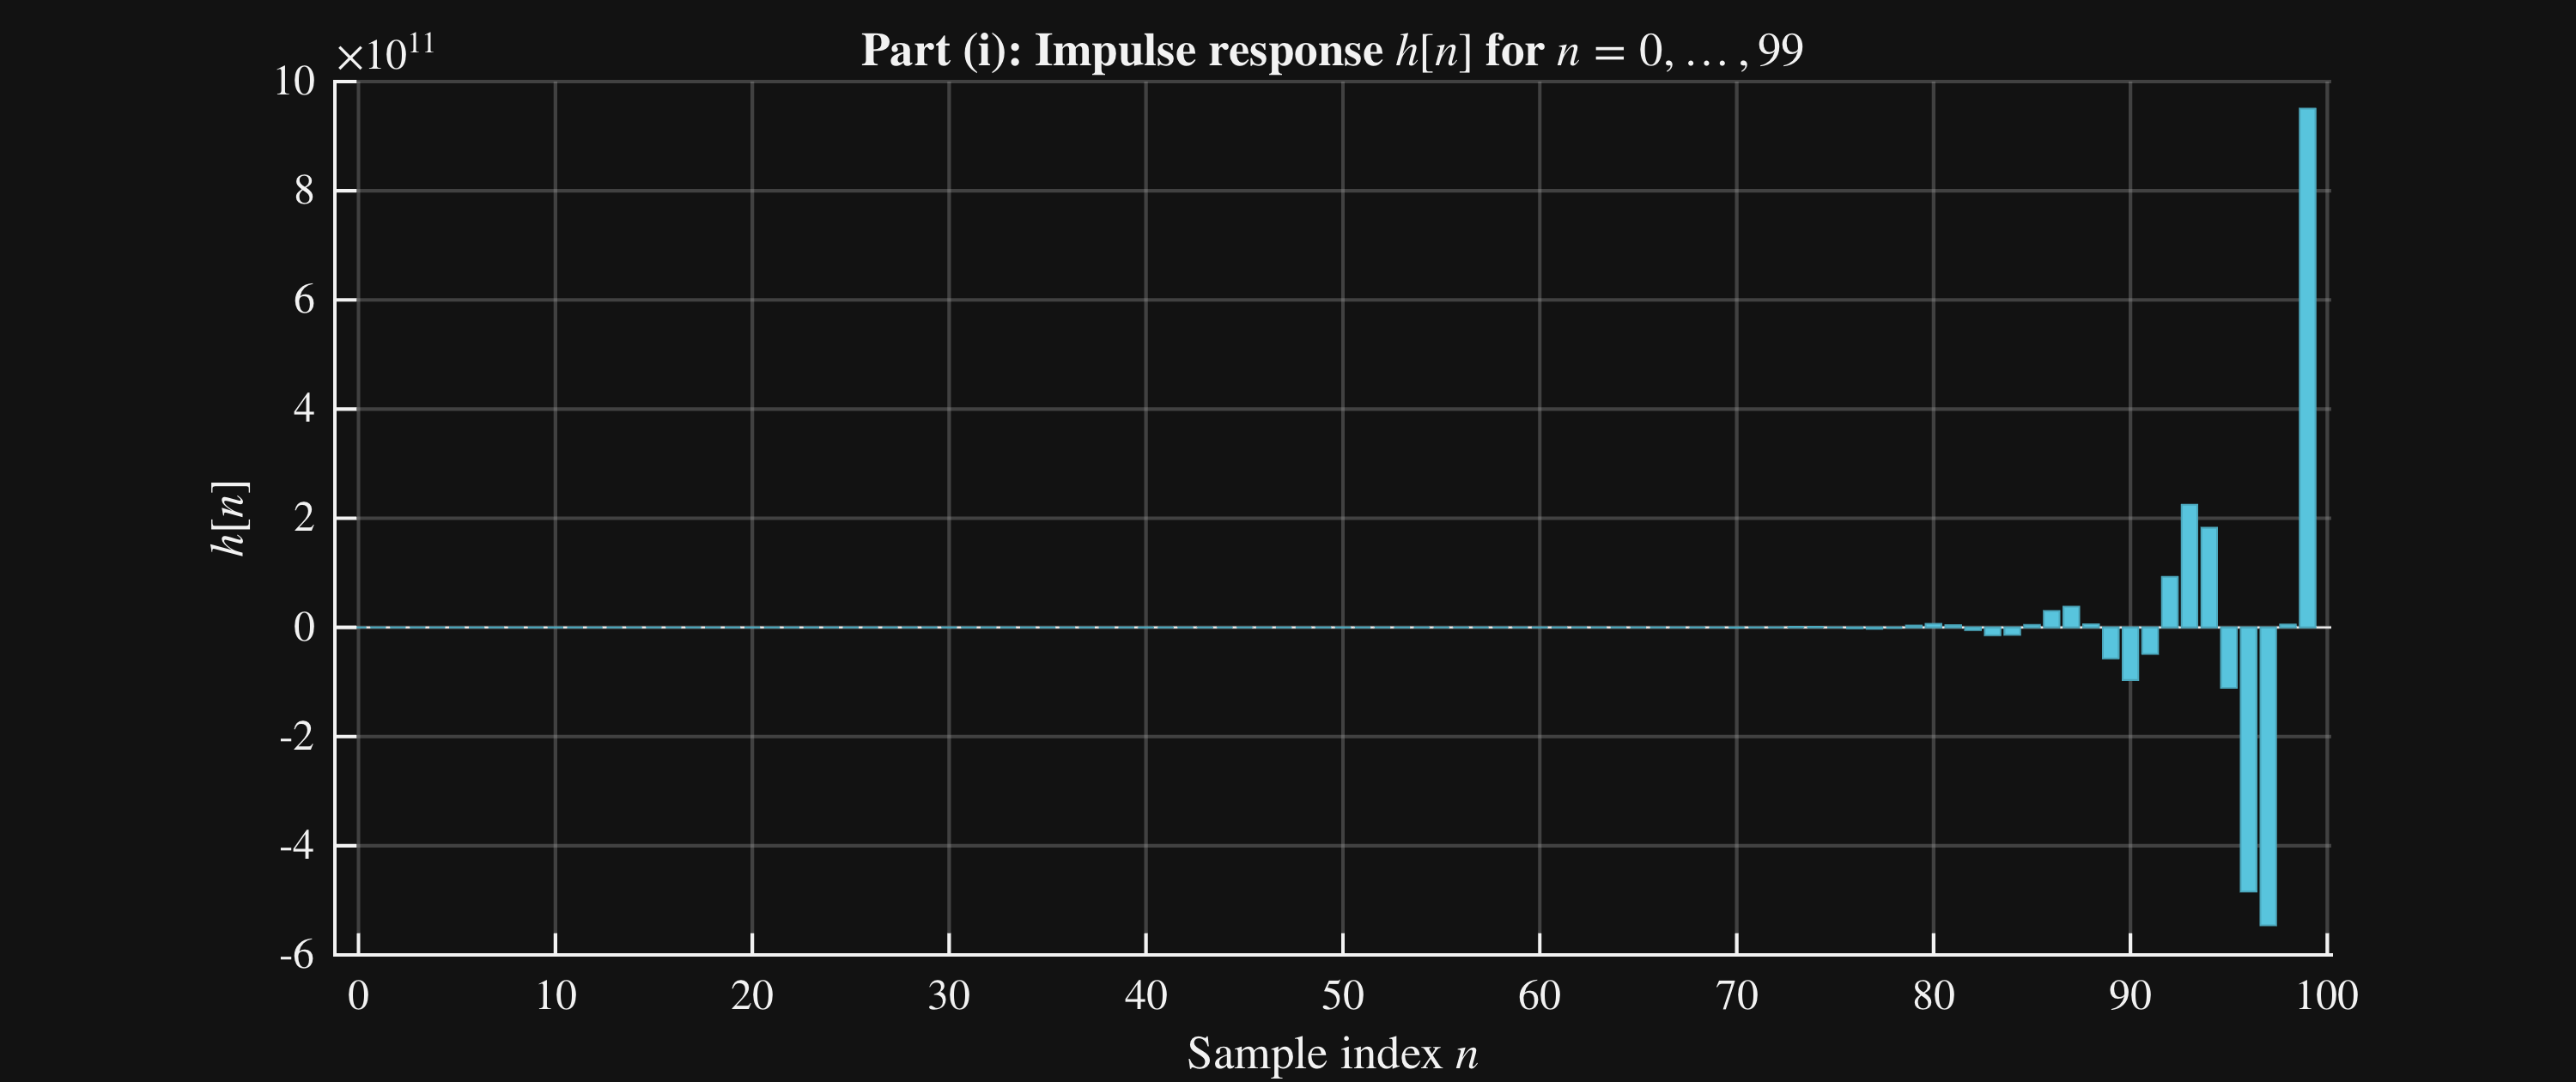
\includegraphics[width=0.96\linewidth]{figures/part1_impulse_response.png}
\captionof{figure}{Open-loop impulse response \(h[n]\) for \(n=0,\dots,99\).}
\end{figurePanel}

\begin{noteBox}
The bar plot already suggests that the response is not decaying to zero. Instead, the magnitude grows, which is a warning sign of instability.
\end{noteBox}
\end{solution}

% ============================================================
% PART (ii)
% ============================================================
\sectionheader{Part (ii): Pole-Zero Plot and Stability}

\begin{problem}{ii}
Use the zero-pole plot of \(H(z)\) and compute the poles of \(H(z)\). Let \(R_{\max}\) be the magnitude of the outermost pole. Confirm that
\[
\log_{10}(R_{\max})\approx \frac{40}{N_{\text{ceil}}}.
\]
Why is this approximation valid?
\end{problem}

\begin{solution}{ii}
The poles are the roots of
\[
6z^4-9z^3+9z^2+2z-2=0.
\]
Numerically, the largest pole magnitude is
\[
\boxed{R_{\max}\approx 1.314446.}
\]
Since \(R_{\max}>1\), at least one pole lies outside the unit circle, so the system is \textbf{BIBO unstable}.

\begin{figurePanel}
\centering
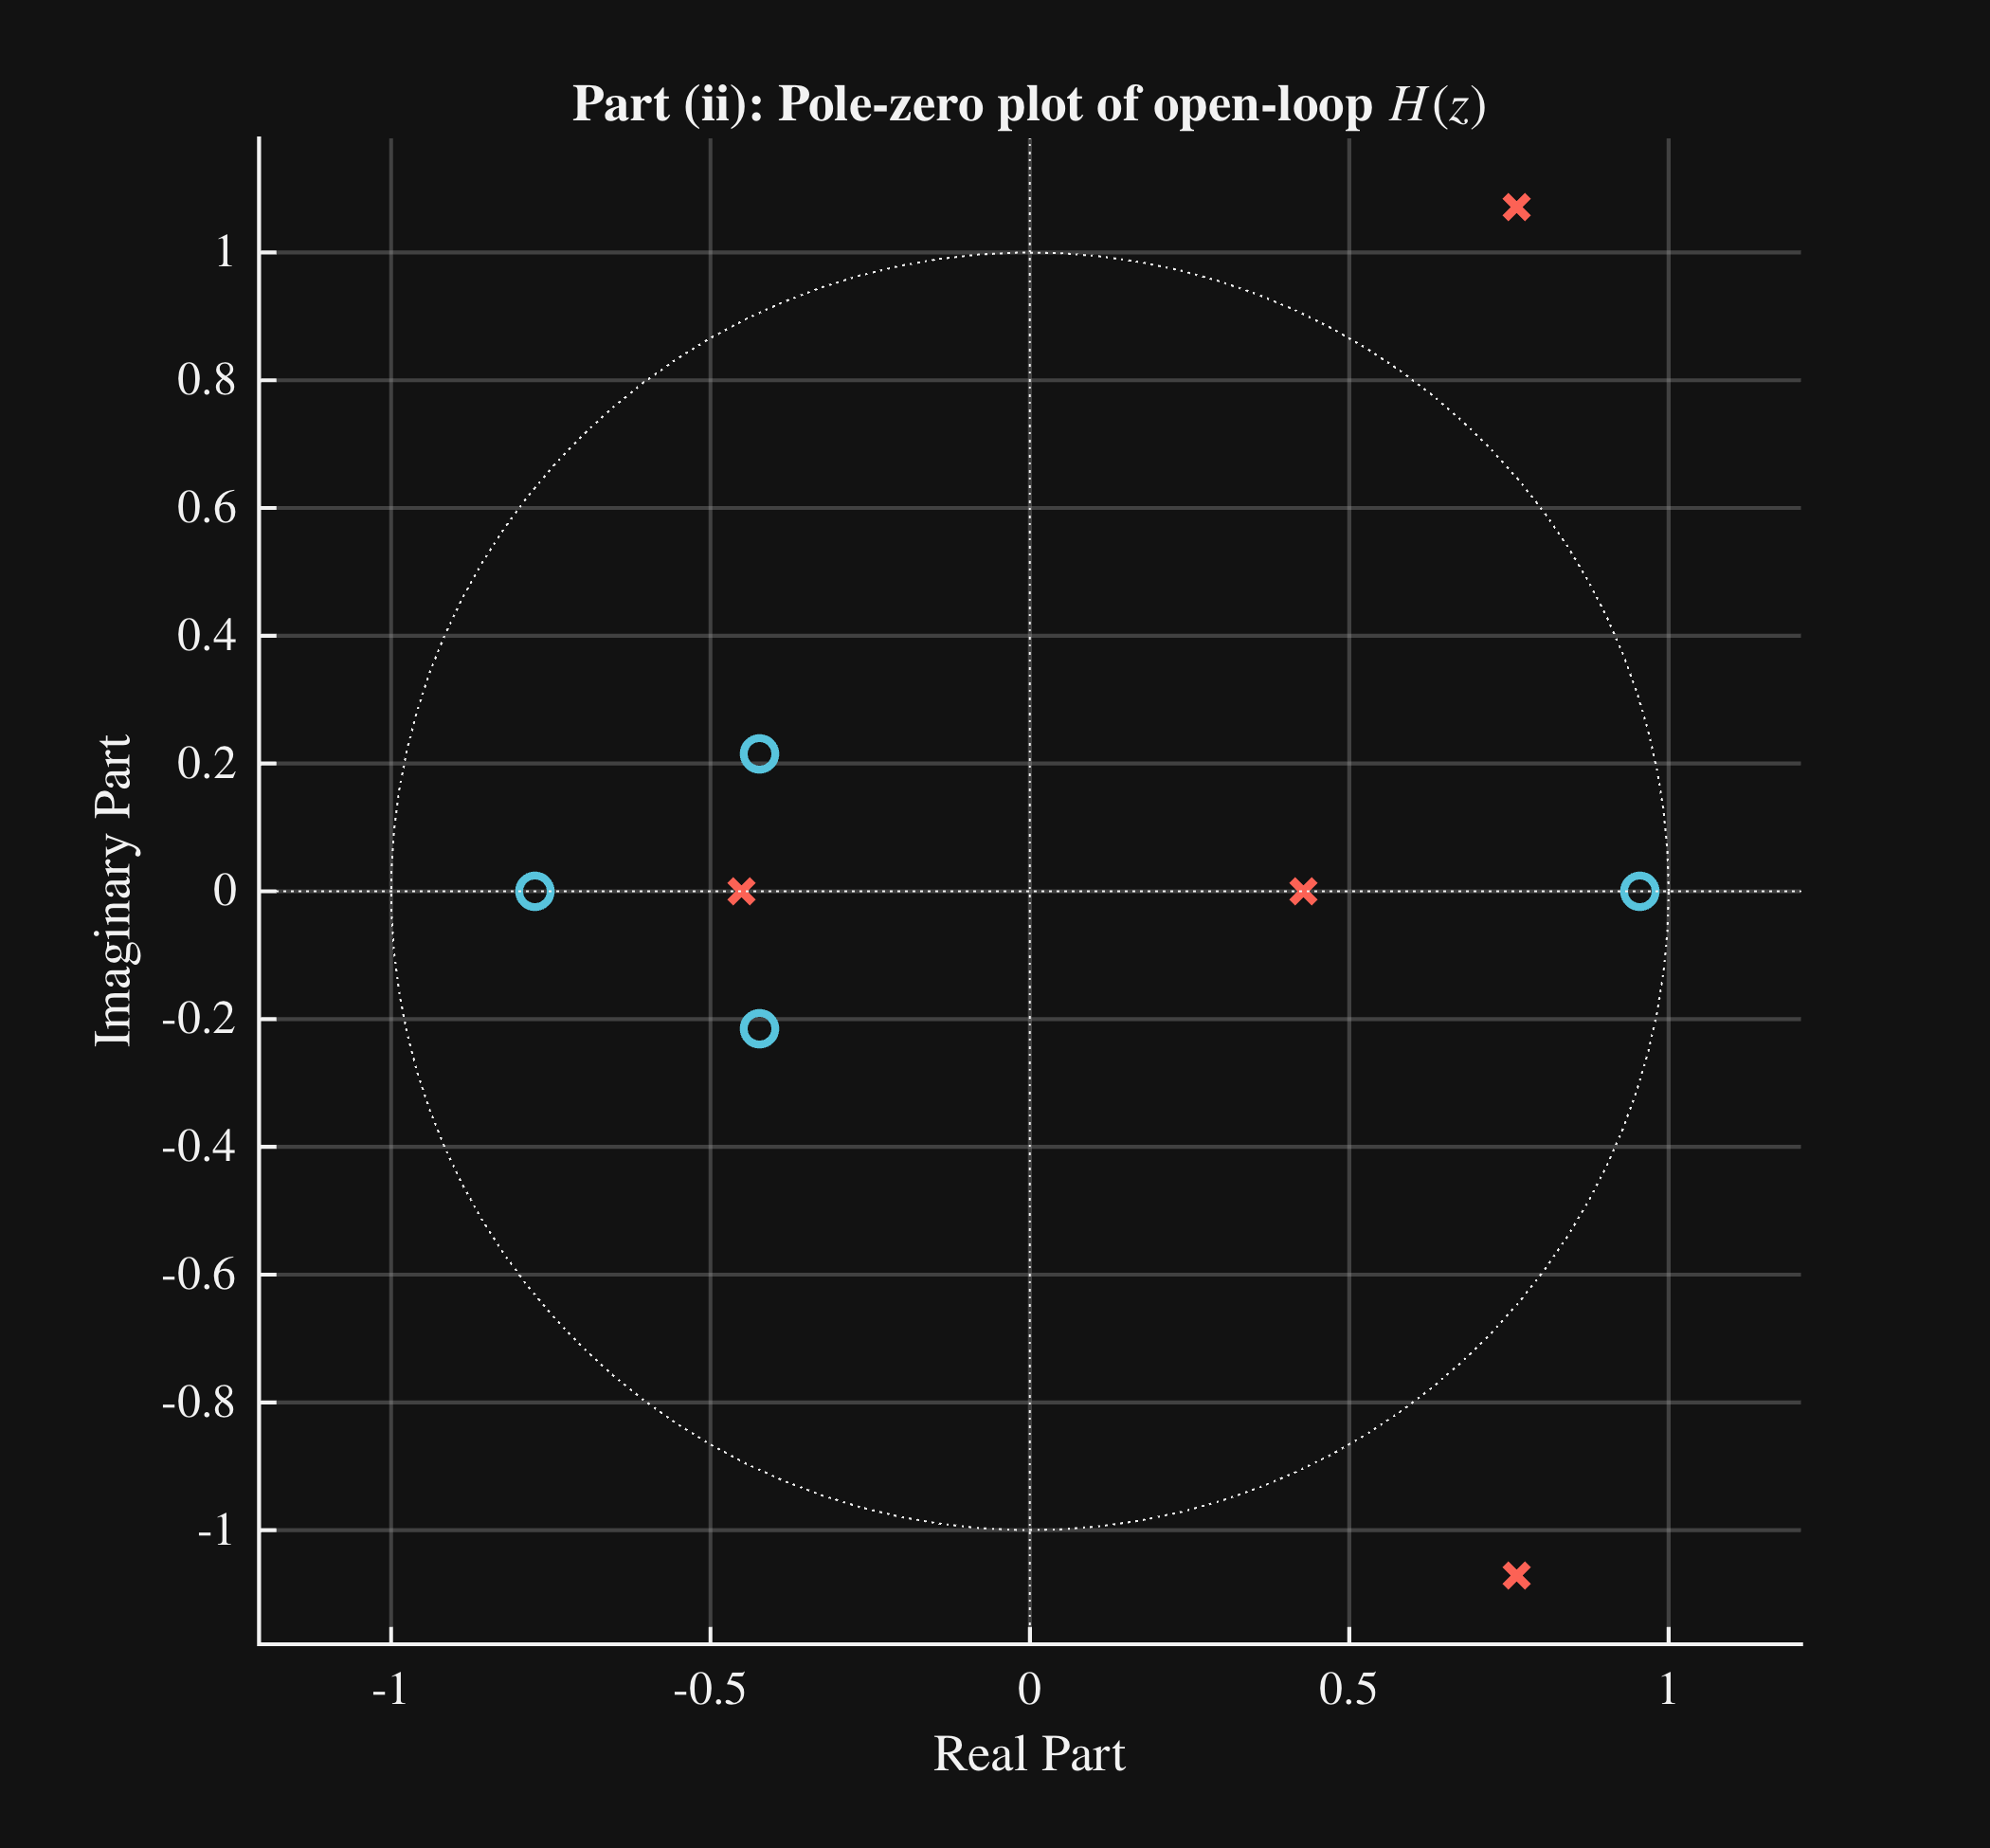
\includegraphics[width=0.72\linewidth]{figures/part2_pole_zero_plot.png}
\captionof{figure}{Pole-zero plot of the open-loop transfer function \(H(z)\).}
\end{figurePanel}

Now compare the two quantities:
\[
\log_{10}(R_{\max}) \approx \log_{10}(1.314446)\approx 0.118743,
\]
and
\[
\frac{40}{N_{\text{ceil}}}\approx \frac{40}{336}\approx 0.119048.
\]
These are very close, which confirms the approximation.

\begin{noteBox}
This works because for large \(n\), the impulse response is dominated by the pole with largest magnitude. So \(h[n]\) behaves roughly like \(C(R_{\max})^n\). When \(|h[n]|\) reaches about \(10^{40}\), we have
\[
(R_{\max})^{N_{\text{ceil}}}\approx 10^{40}.
\]
Taking \(\log_{10}\) gives
\[
N_{\text{ceil}}\log_{10}(R_{\max})\approx 40,
\]
which leads to
\[
\log_{10}(R_{\max})\approx \frac{40}{N_{\text{ceil}}}.
\]
\end{noteBox}

Therefore,
\[
\boxed{\text{The open-loop filter is BIBO unstable.}}
\]
\end{solution}

% ============================================================
% PART (iii)
% ============================================================
\sectionheader{Part (iii): Closed-Loop System Function}

\begin{problem}{iii}
For the feedback configuration with gain \(K>0\), write the closed-loop system function
\[
G(z)=\frac{Y(z)}{X(z)}
\]
in the standard form \(B(z)/A(z)\).
\end{problem}

\begin{solution}{iii}
From the diagram, the feedback is \textbf{negative feedback}, so the signal entering the filter is
\[
E(z)=X(z)-K\,Y(z).
\]
Since
\[
Y(z)=H(z)E(z),
\]
we get
\[
Y(z)=H(z)\bigl(X(z)-K\,Y(z)\bigr).
\]
Rearranging,
\[
Y(z)\bigl(1+K H(z)\bigr)=H(z)X(z).
\]
Hence
\[
G(z)=\frac{Y(z)}{X(z)}=\frac{H(z)}{1+K H(z)}.
\]
Using \(H(z)=B(z)/A(z)\),
\[
G(z)=\frac{B(z)}{A(z)+K B(z)}.
\]

So the closed-loop numerator is still
\[
B(z)=6+4z^{-1}-4z^{-2}-4z^{-3}-z^{-4},
\]
and the closed-loop denominator is
\[
A_{\text{cl}}(z)=A(z)+K B(z).
\]
Therefore,
\[
\boxed{
G(z)=
\frac{6+4z^{-1}-4z^{-2}-4z^{-3}-z^{-4}}
{(6+6K)+(-9+4K)z^{-1}+(9-4K)z^{-2}+(2-4K)z^{-3}+(-2-K)z^{-4}}
}.
\]
\end{solution}

% ============================================================
% PART (iv)
% ============================================================
\sectionheader{Part (iv): Find the Smallest Stabilizing Gain}

\begin{problem}{iv}
Determine the smallest value of \(K\), accurate to three decimal digits, such that the closed-loop system is BIBO stable.
\end{problem}

\begin{solution}{iv}
For BIBO stability, all poles of the closed-loop transfer function must lie strictly inside the unit circle. So the denominator
\[
A_{\text{cl}}(z)=A(z)+K B(z)
\]
was checked as \(K\) varied over the interval \([0,5]\).

The plot below shows the maximum pole magnitude \(R_{\max}\) of the closed-loop system as a function of \(K\).

\begin{figurePanel}
\centering
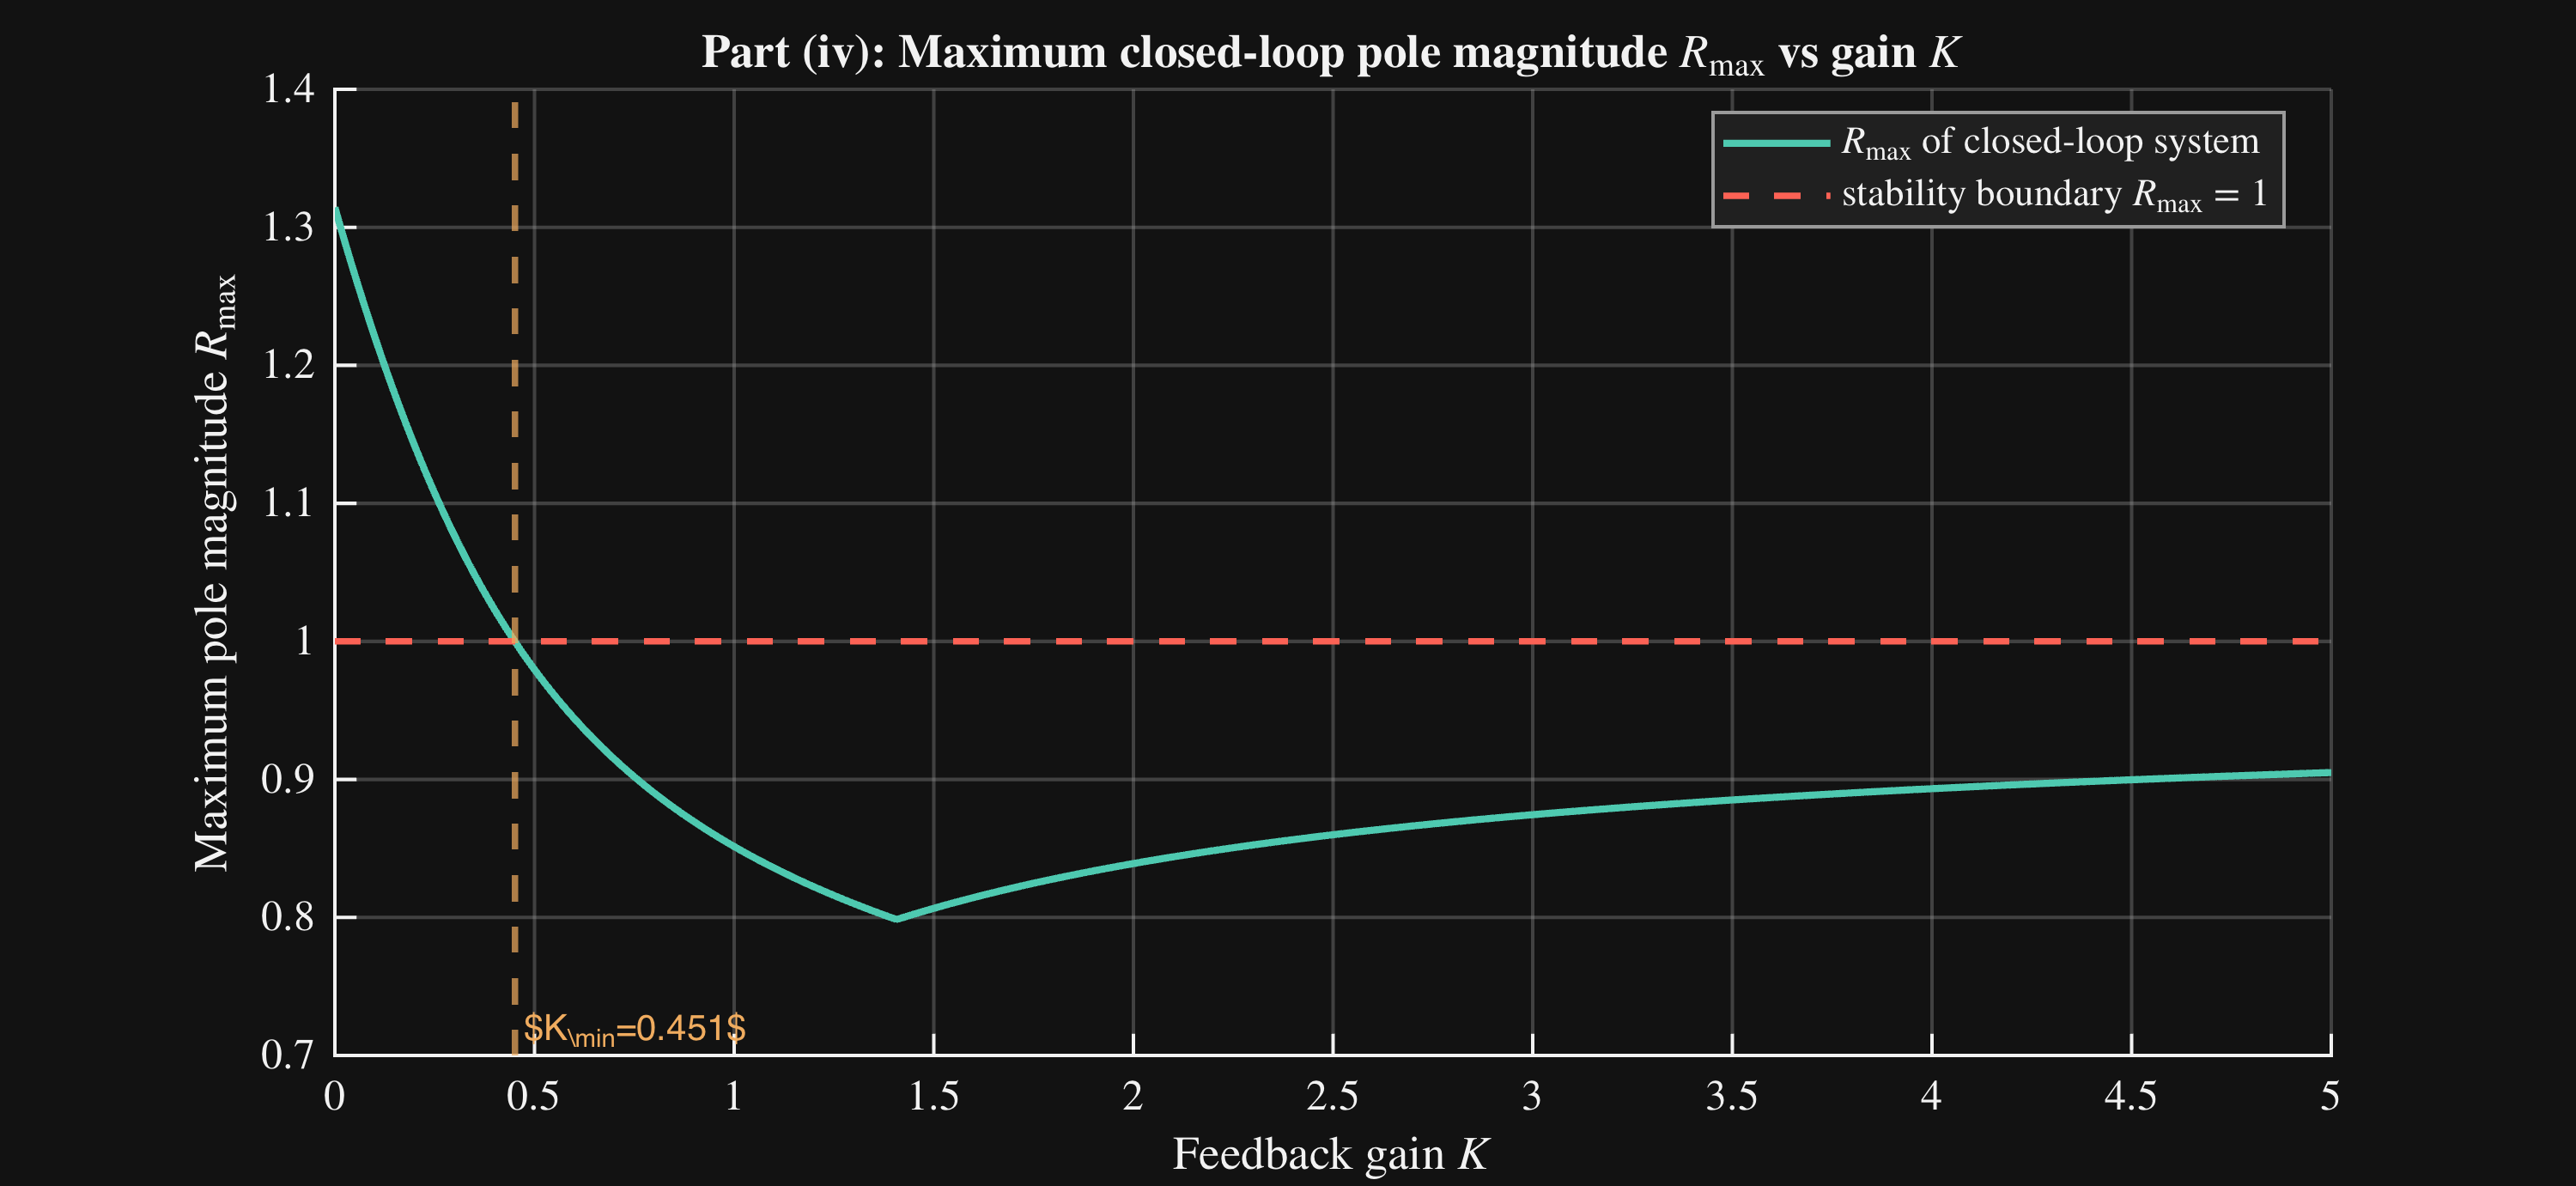
\includegraphics[width=0.96\linewidth]{figures/part4_stability_vs_K.png}
\captionof{figure}{Maximum closed-loop pole magnitude versus gain \(K\). Stability occurs when \(R_{\max}<1\).}
\end{figurePanel}

The first value of \(K\) for which the closed-loop poles move inside the unit circle is
\[
\boxed{K_{\min}=0.451.}
\]

Thus, the smallest gain accurate to three decimal places that stabilizes the system is
\[
\boxed{K=0.451.}
\]
\end{solution}

% ============================================================
% PART (v)
% ============================================================
\sectionheader{Part (v): Closed-Loop Impulse Response}

\begin{problem}{v}
Using the stabilizing value of \(K\) found in part (iv), compute the closed-loop impulse response \(g[n]\) for \(n=0:999\). Plot it as a continuous graph and confirm that the oscillations decay.
\end{problem}

\begin{solution}{v}
Using
\[
\boxed{K=0.451,}
\]
the closed-loop system is stable, so its impulse response should decay as \(n\to\infty\).

The impulse response \(g[n]\) for \(n=0,\dots,999\) is shown below.

\begin{figurePanel}
\centering
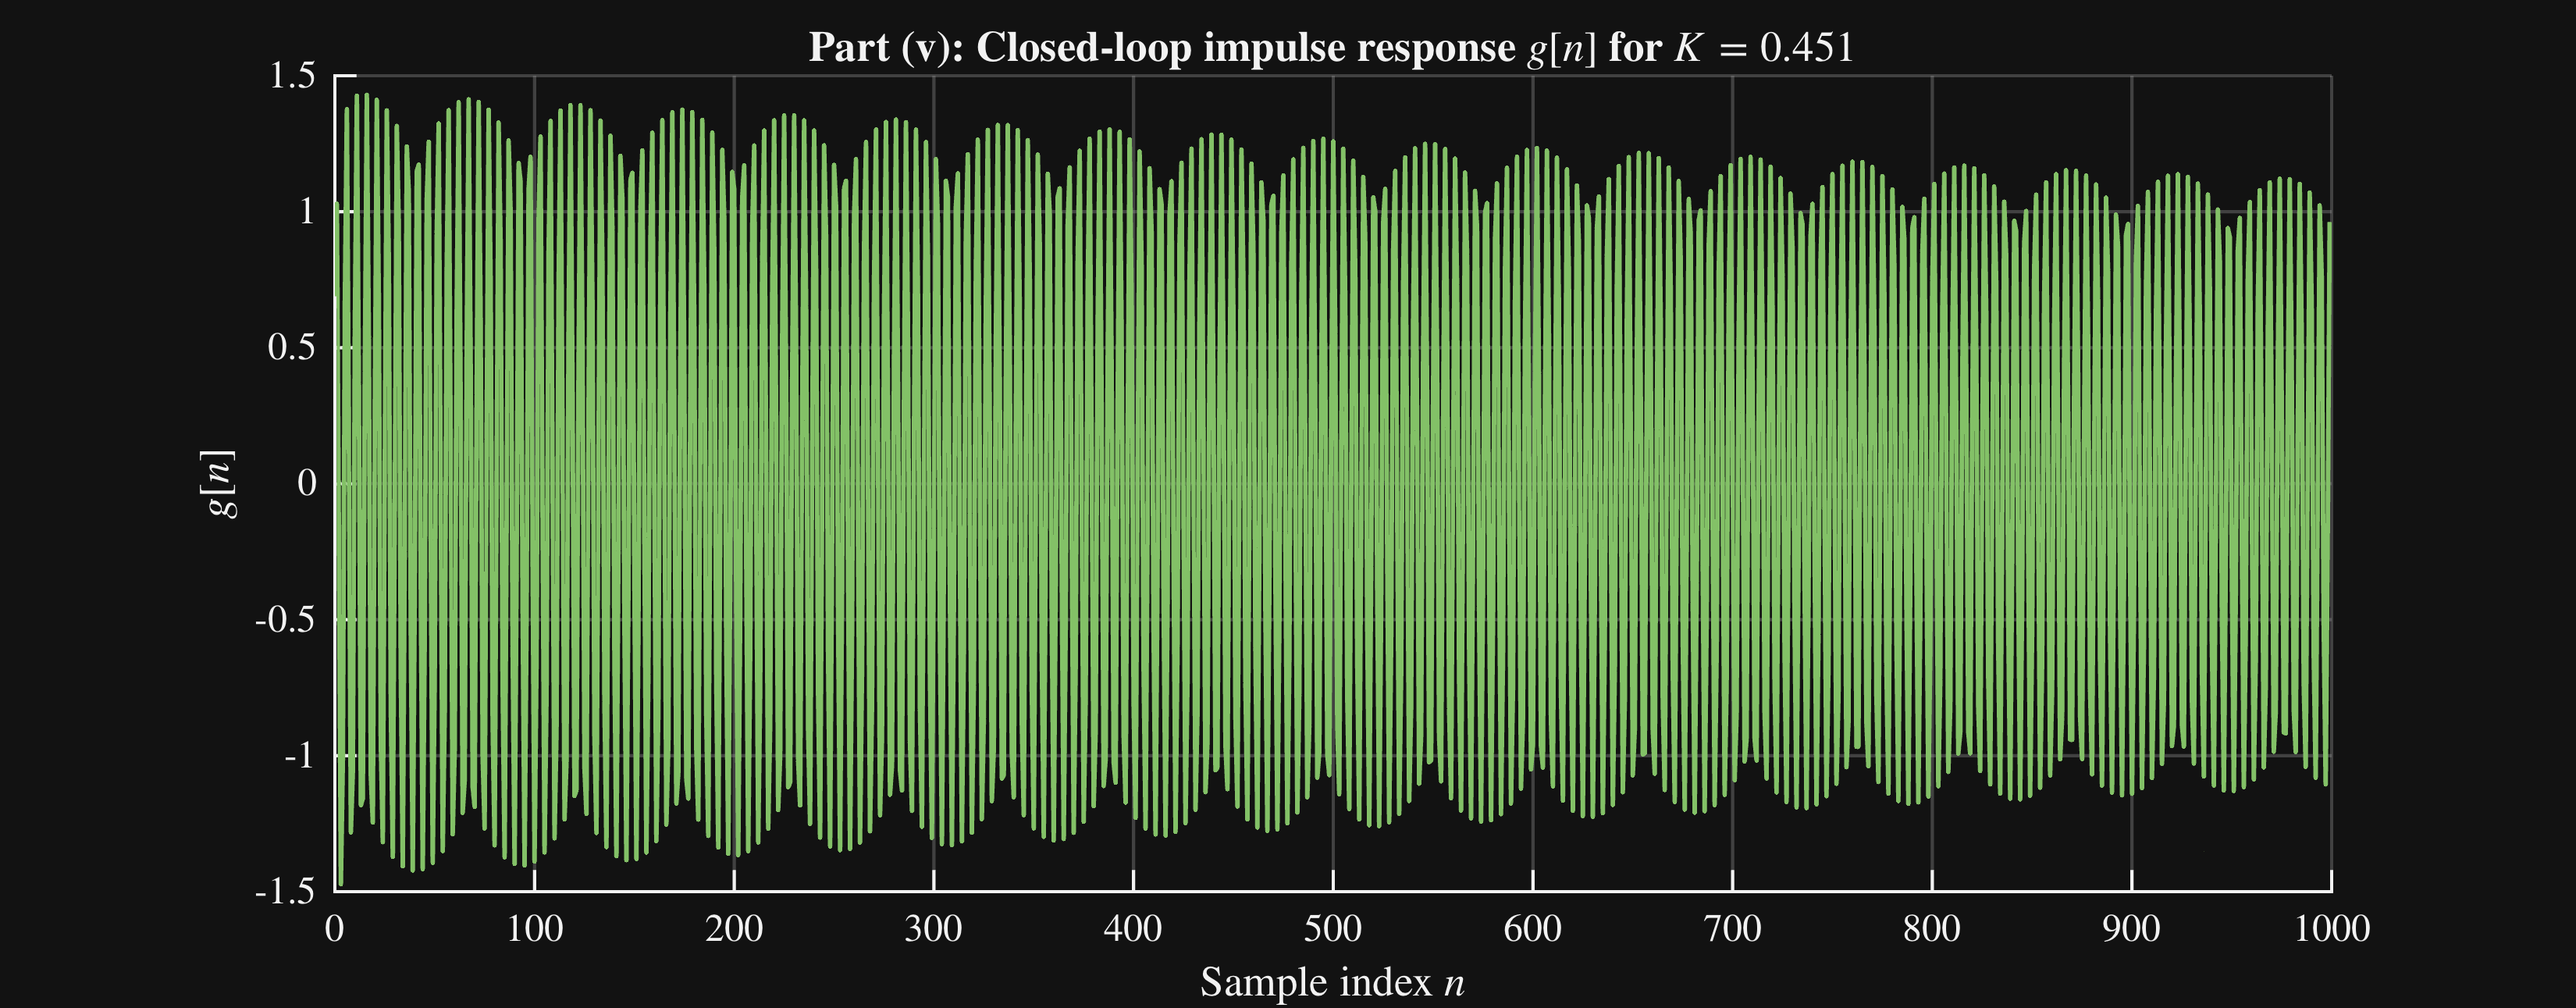
\includegraphics[width=0.96\linewidth]{figures/part5_closed_loop_impulse_response.png}
\captionof{figure}{Closed-loop impulse response \(g[n]\) for \(K=0.451\).}
\end{figurePanel}

To make the decay easier to see, the magnitude \(|g[n]|\) is also plotted on a logarithmic scale.

\begin{figurePanel}
\centering
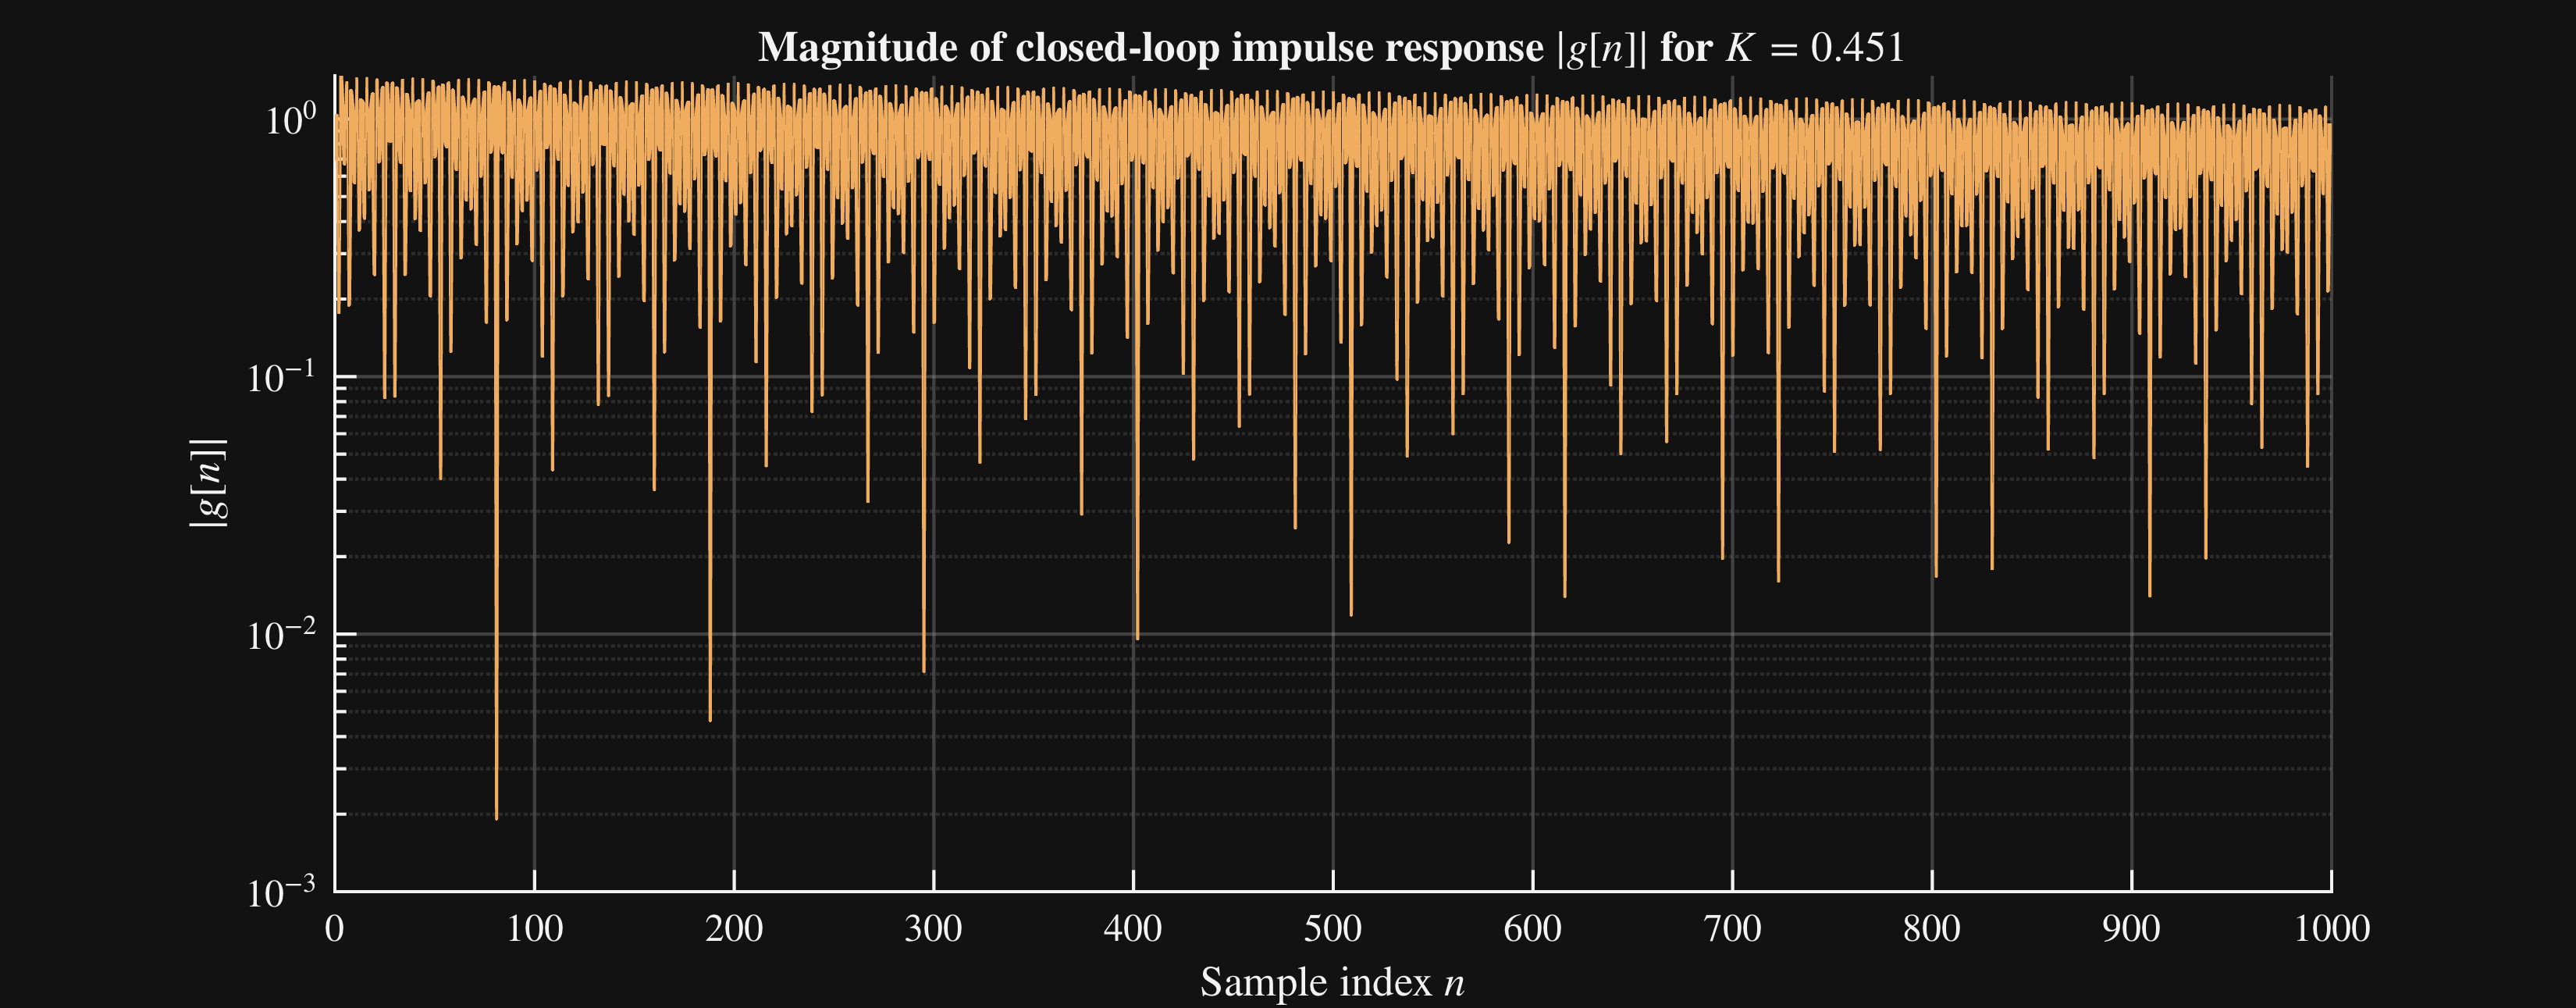
\includegraphics[width=0.96\linewidth]{figures/part5_closed_loop_impulse_magnitude.png}
\captionof{figure}{Magnitude of the closed-loop impulse response on a log scale.}
\end{figurePanel}

The oscillations clearly decay as \(n\) increases, which confirms that the closed-loop system is BIBO stable when
\[
\boxed{K=0.451.}
\]
\end{solution}

% ============================================================
% FINAL SUMMARY
% ============================================================
\sectionheader{Final Answers}

\begin{tcolorbox}[sharp corners, borderline west={2.6pt}{0pt}{TEAL}, colback=PANEL2]
\[
\boxed{N_{\text{ceil}}\approx 336}
\]

\vspace{1mm}
\[
\boxed{R_{\max}\approx 1.314446}
\]

\vspace{1mm}
\[
\boxed{\log_{10}(R_{\max})\approx \frac{40}{N_{\text{ceil}}}}
\]

\vspace{1mm}
\[
\boxed{
G(z)=\frac{H(z)}{1+K H(z)}=\frac{B(z)}{A(z)+K B(z)}
}
\]

\vspace{1mm}
\[
\boxed{K_{\min}=0.451}
\]
\end{tcolorbox}

\vspace{10mm}
\begin{center}
  {\color{GRAY}\rule{12cm}{1.2pt}}\\[6pt]
  {\color{BLUE}\Large End of Project Writeup}
\end{center}

\end{document}